\documentclass[conference]{IEEEtran}
\IEEEoverridecommandlockouts

\usepackage[pdftex,pdfpagelabels,bookmarks,hyperindex,hyperfigures]{hyperref}

\usepackage{float}
\usepackage{adjustbox}
\usepackage[table]{xcolor}
\usepackage{cite}
\usepackage{tikz}
\usetikzlibrary{arrows.meta,
                matrix,
                positioning}
\usepackage{amsmath,amssymb,amsfonts}
\usepackage{algorithmic}
\usepackage{graphicx}
\usepackage{textcomp}
\usepackage{xcolor}
\def\BibTeX{{\rm B\kern-.05em{\sc i\kern-.025em b}\kern-.08em
    T\kern-.1667em\lower.7ex\hbox{E}\kern-.125emX}}
% \usepackage[margin=0.25in]{geometry}
% \usepackage{geometry}
\usepackage{pgfplots}
\pgfplotsset{compat=1.9}
% \pgfplotsset{width=7cm,height=5cm,compat=newest}

\begin{document}

\title{3P71 Assignment 2\\}

\author{
    \IEEEauthorblockN{Parker TenBroeck 7376726}
    pt21zs@brocku.ca
}
\maketitle

\section{Introduction}
This document shows the performance of a GA system designed to solve the scheduling problem outlined in the assignment. The solution implementation will be tested with varying parameters and problem sets to show what configurations product the best results and how they compare to each other.

\subsection{The Problem}
A university has been tasked with creating a program to assign courses which have professors teaching them to rooms and timeslots while satisfying multiple constraints. We know that a course must be scheduled in a room with space for at least the number of students in that course, if not more. A room which is booked at a certain timeslot for one course cannot be scheduled any other course at that timeslot. And finally a professor traching one course cannot be scheduled to teach another course(or the same course) at the same time. It has been decided that a genetic algorithm is the best method for solving this problem.

\section{GA Overview}
A GA system is a way to represent and solve particular problems by representing potential solutions as chromosomes, who we call individuals. These chromosomes are made of genes which represent individual parts of a potential solution which we can change. Individuals exist in a population where each new generation we apply algorithms to better our potential solutions, hoping to converge on a satisfactory answer\cite[p. 3]{ga-tut1}. \vspace{8pt}

In A GA system there are five important algorithms to consider, Fitness, Elitism, Selection, Crossover, and Mutation \cite[p. 6]{ga-tut1}. \vspace{8pt}

Fitness determines how individuals are evaluated, and gives us a ranking of "best" to "worst". We can also use fitness to help determine if a particular individual is a satisfactory solution.\vspace{8pt}

Elitism determines how many of the top $k$ members of the population will be guaranteed in the next population. These individuals won't be mutated in any way \cite[p. 7]{ga-tut1}.\vspace{8pt}

Selection determines how members of a previous population are selected for the new population. Selection happens after we copy the elites from the previous population filling the remaining population with individuals decided by selection\cite[p. 9]{ga-tut1}. \vspace{8pt}

Crossover determines how two individuals will 'breed' that is, how two individuals genes are combined to create two children whos genes are some combination of their parents. There is a associated percentage for crossover that determines the chance any given chromosome will have individual applied to it\cite[p. 12]{ga-tut1}.\vspace{8pt}

Finally mutation determines how chromosomes are mutated, specifically how individual genes are mutated inside any particular chromosome. mutation also has a probability associated with it which is the percent change a given individual will undergo mutation.\vspace{8pt}

The GA implemented was based off these slides \cite{ga-tut1}.

\subsection{Fitness}
Fitness determines how "fit" any individual is, that is gives us a numeric way of raking individuals against each other. In our case our fitness is determined by the reciprocal of a weighed sum over the number of different conflicts present in a schedule


\begin{gather}
C=\text{Over room capacity} \notag\\
R=\text{Room overbooked in timeslot} \notag\\
P=\text{Professor overbooked in timeslot} \notag\\
\text{raw}=3C+2R+P\label{raw}\\
\text{normalized}=\frac{1}{1+\text{raw}}\label{normalized}
\end{gather}

\subsection{Selection}
In this GA there is only a single algorithm for selection. It is $K$ Tournament selection. For every remaining slot in the population that wasn't filled by elitism the selection algorithm runs. The algorithm simply selects $K$ individuals from the previous population and gives the best individual of those $K$. in our case $K=4$ so 4 individuals are selected from the old population, and the best of the $4$ in terms of fitness is selected for that slot. This is repeated until every slot in the new population is filled.   


\subsection{Mutation}
Similarly to selection there is only one algorithm for mutation. The algorithm simply chooses a random gene, and replaces it with a new random, but possible gene. Mutation is attempted on all individuals in a population except elitism individuals. for every individual in a generation there is a percent chance mutation happen, this is determined by the mutation rate parameter. 

\subsection{Crossover}
Crossover can occurs between two individuals that were selected in the selection step. how often crossover happens is determined by the crossover rate parameter. If two individuals aren't selected then they are directly placed in the population. If they are then the specified crossover algorithm is ran on them and their resulting children are placed in the new population. Crossover does not mutate the elitism individuals. There are three available crossover algorithms, two are from class, one is a custom crossover operator designed specifically for this problem.

\subsubsection{One Point Crossover} This crossover works by selecting a random index $i$ and swapping all genes after $i$ \cite[p. 17]{ga-tut1}. 
\begin{center}
    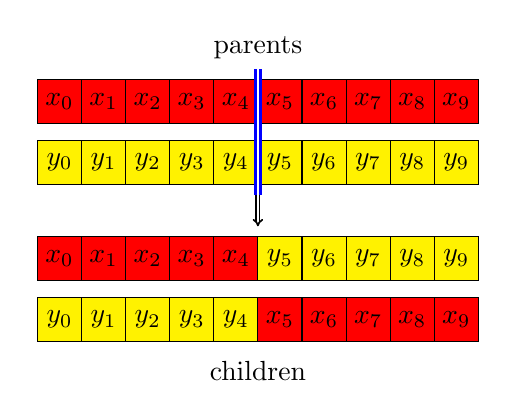
\begin{tikzpicture}[
node distance = 4mm,
  MTRX/.style = {matrix of nodes,
                 nodes={draw, minimum size=5.6mm, anchor=center,
                        inner sep=0pt, outer sep=0pt},
                 column sep=-\pgflinewidth,
                 row sep=2mm},
    CR/.style = {fill=red},  %fill  Color Red
    CY/.style = {fill=yellow}%fill  Color Yellow
                        ] 
% left table
\matrix  (m1) [MTRX,
               row 1/.append style = {nodes={CR}},
               row 2/.append style = {nodes={CY}},
               label=above: parents
               ] 
{
$x_0$ & $x_1$ & $x_2$ & $x_3$ & $x_4$ & $x_5$ & $x_6$ & $x_7$ & $x_8$ & $x_9$\\
$y_0$ & $y_1$ & $y_2$ & $y_3$ & $y_4$ & $y_5$ & $y_6$ & $y_7$ & $y_8$ & $y_9$\\
};
% right table
\matrix  (m2) [MTRX, below=of m1,
               label=below:children
               ]
{
  |[CR]| $x_0$ & |[CR]| $x_1$ & |[CR]| $x_2$ & |[CR]| $x_3$ & |[CR]| $x_4$
& |[CY]| $y_5$ & |[CY]| $y_6$ & |[CY]| $y_7$ & |[CY]| $y_8$ & |[CY]| $y_9$   \\
  |[CY]| $y_0$ & |[CY]| $y_1$ & |[CY]| $y_2$ & |[CY]| $y_3$ & |[CY]| $y_4$
& |[CR]| $x_5$ & |[CR]| $x_6$ & |[CR]| $x_7$ & |[CR]| $x_8$ & |[CR]| $x_9$   \\
};
\draw[very thick, blue, double] (m1.north) -- (m1.south);
\draw[double, -{Implies[]}, semithick] (m1.south) -- (m2.north);
\end{tikzpicture}

\end{center}

\subsubsection{Uniform Crossover} This crossover randomly swaps genes at any given point. Each swap has an equal 50\% chance of occurring \cite[p. 21-29]{ga-tut1}.
\begin{center}
    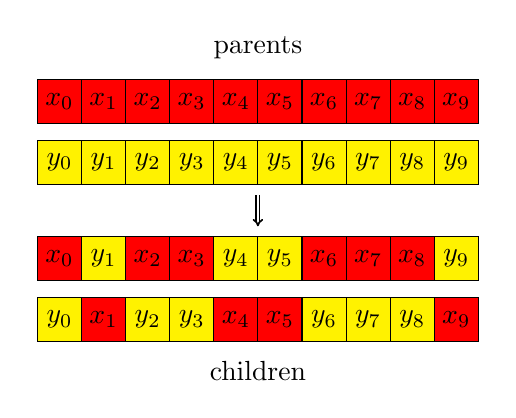
\begin{tikzpicture}[
node distance = 4mm,
  MTRX/.style = {matrix of nodes,
                 nodes={draw, minimum size=5.6mm, anchor=center,
                        inner sep=0pt, outer sep=0pt},
                 column sep=-\pgflinewidth,
                 row sep=2mm},
    CR/.style = {fill=red},  %fill  Color Red
    CY/.style = {fill=yellow}%fill  Color Yellow
                        ] 
% left table
\matrix  (m1) [MTRX,
               row 1/.append style = {nodes={CR}},
               row 2/.append style = {nodes={CY}},
               label=above: parents
               ] 
{
$x_0$ & $x_1$ & $x_2$ & $x_3$ & $x_4$ & $x_5$ & $x_6$ & $x_7$ & $x_8$ & $x_9$\\
$y_0$ & $y_1$ & $y_2$ & $y_3$ & $y_4$ & $y_5$ & $y_6$ & $y_7$ & $y_8$ & $y_9$\\
};
% right table
\matrix  (m2) [MTRX, below=of m1,
               label=below:children
               ]
{
  |[CR]| $x_0$ & |[CY]| $y_1$ & |[CR]| $x_2$ & |[CR]| $x_3$ & |[CY]| $y_4$
& |[CY]| $y_5$ & |[CR]| $x_6$ & |[CR]| $x_7$ & |[CR]| $x_8$ & |[CY]| $y_9$   \\
  |[CY]| $y_0$ & |[CR]| $x_1$ & |[CY]| $y_2$ & |[CY]| $y_3$ & |[CR]| $x_4$
& |[CR]| $x_5$ & |[CY]| $y_6$ & |[CY]| $y_7$ & |[CY]| $y_8$ & |[CR]| $x_9$   \\
};
\draw[double, -{Implies[]}, semithick] (m1.south) -- (m2.north);
\end{tikzpicture}

\end{center}

\subsubsection{Best Attempt Crossover}
This crossover attempts to minimize the number of conflicts per gene swap. It starts with the first gene and at every gene $i$ it chooses the configuration that has the least conflicts. If the number of conflicts are the same there is a 50\% chance of a particular pair of genes swapping or not. This continues for all genes in the chromosome. 

\begin{center}
    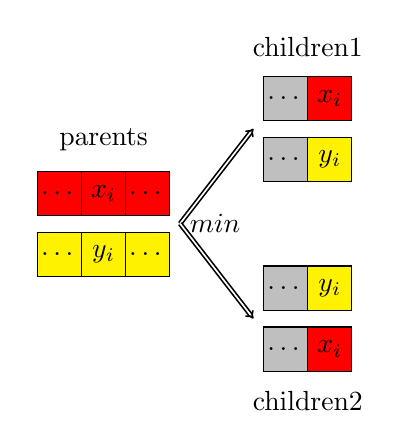
\begin{tikzpicture}[
node distance = 4mm,
  MTRX/.style = {matrix of nodes,
                 nodes={draw, minimum size=5.6mm, anchor=center,
                        inner sep=0pt, outer sep=0pt},
                 column sep=-\pgflinewidth,
                 row sep=2mm},
    CR/.style = {fill=red},  %fill  Color Red
    CY/.style = {fill=yellow},%fill  Color Yellow
    CG/.style = {fill=lightgray}%fill  Color Yellow
                        ] 
% left table
\matrix  (m1) [MTRX,
               row 1/.append style = {nodes={CR}},
               row 2/.append style = {nodes={CY}},
               label=above: parents,
               label=right: \space $min$
               ] 
{
\ldots & $x_i$ & \ldots \\
\ldots & $y_i$ & \ldots \\
};
\matrix  (mm) [MTRX, right=of m1]{\\};
\matrix  (m2) [MTRX, above right=of mm,
               label=above:children1
               ]
{
  |[CG]| \ldots & |[CR]| $x_i$   \\
  |[CG]| \ldots & |[CY]| $y_i$   \\
};
\matrix  (m3) [MTRX, below right=of mm,
               label=below:children2
               ]
{
  |[CG]| \ldots & |[CY]| $y_i$   \\
  |[CG]| \ldots & |[CR]| $x_i$   \\
};
\draw[double, -{Implies[]}, semithick] (m1.east) -- (m2.west);
\draw[double, -{Implies[]}, semithick] (m1.east) -- (m3.west);
\end{tikzpicture}

\end{center}

This method was specifically implemented for this problem as it is fairly trivial to test which set of children will have a better fitness at every step allowing us to take a greedy approach that gives significant gains. In the cases where the locally optimal choice isn't the overall optimal choice mutation and genetic diversity keeps the GA system from getting stuck in a local maximum. 

\section{Setup}
\subsection{Compilation}
In the provided code there is a shell script \texttt{build.sh} which when ran compiles all the code and creates a jar called \texttt{assign2.jar}. 

\subsection{Running}
Running the program can be done with \texttt{java -jar assign2.jar} and configuring the CLI args. \texttt{<num>} is a integer, \texttt{<rate>} is a percentage value from 0-1. The problem set and generations number must be given, and the seeds must be set using one of the methods below.\\\\
\small
\texttt{-{}-problem-set <path>}: the path to the problem set\\
\texttt{-{}-seeds-linear <num>}: sets the seeds to 0 to $<$num$>$-1\\
\texttt{-{}-seeds-rand <num>}: creates $<$num$>$ random seeds\\
\texttt{-{}-seeds +<num,>}: a comma separated list of seeds\\
\texttt{-{}-generations <num>}: sets the max number of generations\\
\texttt{-{}-gui}: show the graph GUI.\\
\normalsize
\\
The following parameters will run tests for all permutations of the provided values. These all must have at least one value\\\\
\small
\texttt{-{}-elitism-rates +<num,>}: the elitism rates to test\\
\texttt{-{}-crossover-rates +<rate,>}: the crossover rates to test\\
\texttt{-{}-mutation-rates +<rate,>}: the mutation rates to test\\
\texttt{-{}-initializer-kinds +<kind,>}: the initializer kinds to test\\
\hspace*{10pt}values: \texttt{Random}\\
\texttt{-{}-fitness-kinds +<kind,>}: the fitness kinds to test\\
\hspace*{10pt}values: \texttt{WeightedConflicts}\\
\texttt{-{}-mutation-kinds +<kind,>}: the mutation kinds to test\\
\hspace*{10pt}values: \texttt{SingleGene}\\
\texttt{-{}-crossover-kinds +<kind,>}: the crossover kinds to test\\
\hspace*{10pt}values: \texttt{OnePoint, Uniform, BestAttempt}\\
\normalsize
\vspace{8pt}

There is a shell script \texttt{run\_defaults.sh} which runs all of the tests ran in this document. All you provide is the path to the problem set, and optionally \texttt{-{}-gui} if you wish to display the grahps\vspace{8pt}

the results for each test will be outputed into the directory \texttt{runs} containing a file starting at \texttt{run1.json} through \texttt{run\#.json} which contains all the data collected for every run. \textbf{Important} the directory \texttt{runs} in the CWD will be deleted including its contents upon running the program.

\section{Results}

In all these tests the raw fitness(solid lines) is defined as \eqref{raw}, the closer to zero the better. And the normalized fitness(dotted lines) is defined as \eqref{normalized}, the closer to 100 the better. Each graph shows the max/average/min of the raw and normalized fitness. Because each configuration is ran 50 times with different seeds we take the average over all runs for every generation. If a run finishes before another, the final values it produced are used as the value for all further generations. A vertical line is shown when a particular run finishes with its generation number, seed number and final normalized fitness value.\\

The parameters not listed for each test don't change and are as follows\\\\
elitism rate: 1 individual\footnote{talked to Reginald and said I could use this value as I had already ran my tests using this parameter before he made the announcement}.\\
selection: $k=4$ tournament selection.\\
seeds: 0-49.\\
fitness: weighted sum.\\
mutation: random gene mutation.\\
initialization: random well formed genes.\\

In Fig.~\ref{fig:td1_fitness} and Fig.~\ref{fig:td2_fitness} we can see that all 50 runs in nearly all configurations the GA was able to find a solution in 250 generations. That means comparing on fitness will not lead to any insights on which set of parameters are better. However, we can use the average last generation as a metric as seen in Fig.~\ref{fig:td1_gens} and Fig.~\ref{fig:td2_gens}. This will let us compare which configurations converge on an answer in fewer generations and give us more insight into how different parameters perform against each other.\\

In Fig.~\ref{fig:run_params} shows which config corresponds to which set of parameters.\\


\begin{figure}[H]
\centering
\input{t1/run_params}
\caption{run parameters}
\label{fig:run_params}
\end{figure}

\begin{figure}[H]
\centering
\input{t1/run_fitness}
\caption{Test data 1 solution fitness results}
\label{fig:td1_fitness}
\end{figure}


\begin{figure}[H]
\centering
\input{t1/run_gens}
\caption{Test data 1 generation completed results}
\label{fig:td1_gens}
\end{figure}

\begin{figure}[H]
\centering
\input{t2/run_fitness}
\caption{Test data 2 solution fitness results}
\label{fig:td2_fitness}
\end{figure}


\begin{figure}[H]
\centering
\input{t2/run_gens}
\caption{Test data 2 generation completed results}
\label{fig:td2_gens}
\end{figure}



Starting with the worst performing configuration Fig.~\ref{fig:td2_config1} we can immediately see that 9 of the 50 runs don't complete in the 250 generations. 

\begin{figure}[H]
    \input{t1/run1}
    \caption{Test data 1 config 1}
    \label{fig:td1_config1}
\end{figure}

We can see Fig.~\ref{fig:td2_config1} exhibits some of the same behavior as Fig.~\ref{fig:td1_config1} but with only two outliers.

\begin{figure}[H]
    \centering
    \input{t2/run1}
    \caption{Test data 2 config 1}
    \label{fig:td2_config1}
\end{figure}


Looking at a different configuration we can see that there aren't any runs which didn't finish. But now we can see more closely that while both Fig.~\ref{fig:td1_config6} and Fig.~\ref{fig:td2_config6} use the same configuration of parameters Fig.~\ref{fig:td1_config6} finishes on average at a much later generation than Fig.~\ref{fig:td2_config6}. We can interpret this as the problem set 1 being potentially harder to solve than problem set 2. If we look at Fig.~\ref{fig:td2_gens} and Fig.~\ref{fig:td1_gens} we can compare the average ending generation and notice that yes, for any given configuration the average is lower for problem set 2 compared to problem set 1. 

\begin{figure}[H]
    \centering
    \input{t1/run6}
    \caption{Test data 1 config 6}
    \label{fig:td1_config6}
\end{figure}

\begin{figure}[H]
    \centering
    \input{t2/run6}
    \caption{Test data 2 config 6}
    \label{fig:td2_config6}
\end{figure}


If we take the same parameters over the same problem set and only change the crossover method we can see something interesting. Here in Fig.~\ref{fig:td1_config8} and Fig.~\ref{fig:td1_config14} we have just that. The configuration using \texttt{BestAttempt} crossover has a significantly lower average completed generation compared to Fig.~\ref{fig:td1_config8}. and if we look further we can actually see for all configurations on problem set one using \texttt{BestAttempt} Fig.~\ref{fig:td1_config14}, Fig.~\ref{fig:td1_config13}, Fig.~\ref{fig:td1_config12}, Fig.~\ref{fig:td1_config11}, Fig.~\ref{fig:td1_config10}, and Fig.~\ref{fig:td1_config9} we get a very similar average completed generation. 
\begin{figure}[H]
    \centering
    \input{t1/run8}
    \caption{Test data 1 config 8}
    \label{fig:td1_config8}
\end{figure}
\begin{figure}[H]
    \centering
    \input{t1/run14}
    \caption{Test data 1 config 14}
    \label{fig:td1_config14}
\end{figure}

These points can be proved using statistical analysis. We will be using the two tailed z-test with a level of significance of $0.05$ Our null hypotheses is $H_0: \mu_0=\mu_1$ vs alternative hypothesis $H_1: \mu_0\neq \mu_1$. We can reject $H_0$ when $p<0.05$. What this means is if we reject the null hypothesis $H_0$ we can say the difference in mean generations to complete is statistically significant and one configuration will on average find a solution is less generations. 
\begin{center}
\large
\begin{gather}
Z=\frac{\overline{x_1}-\overline{x_2}}{\sqrt{\frac{\sigma_1^2}{n_1}+\frac{\sigma_2^2}{n_2}}} \label{ZValue}\\
p=1-erf(\frac {|Z|}{\sqrt{2}}) \label{pValue}
\end{gather}
\end{center}


We first calculate the $Z$ value using \eqref{ZValue} for every combination of listed parameter configurations. the mean and standard deviation can be found in tables Fig.~\ref{fig:td1_gens} and Fig.~\ref{fig:td2_gens} for problem set 1 and problem set 2 respectively. $n$ is simply the number of tests ran per configuration, which in our case is always $50$.  \\

We then find $p$ for every respective $Z$ calculated simply by using \eqref{pValue}. \\

Finally once we have $p$ we can test if we can reject our null hypothesis $H_0$. \\

The table cells are colored in according to the following. If we cannot reject the null hypothesis, that is the average completed generation of the two configurations is not statistically significantly different, we color in the cell yellow. If we can reject the null hypotheses we color the cell green if the column configuration has a lower average completed generation and red otherwise.\\

This intends to show us which configurations are equivalent and if not which configuration is better. To simplify, green means column \# configuration is better than row \# configuration. yellow means they're the same, and red means it is worse. \\

These values can be found in tables Fig.~\ref{fig:td1_zvalues}, Fig.~\ref{fig:td1_pvalues}, and Fig.~\ref{fig:td1_compare} for problem set one and Fig.~\ref{fig:td2_zvalues}, Fig.~\ref{fig:td2_pvalues}, and Fig.~\ref{fig:td2_compare} for problem set two. \\


We can see that in both Fig.~\ref{fig:td1_compare} and Fig.~\ref{fig:td2_compare} the configurations who use \texttt{BestAttempt} crossover perform consistently better than other configurations using other crossover methods, and interestingly perform about the same as each other when configured with different crossover rates and mutation rates. We can also see that in problem set 1 configuration 1 performs significantly worse than any other configuration. Also to note configurations 7, 5, and 3 all seemed to have slight improvements over other configurations in both problem sets. To all three configurations had a mutation value of $0\%$.

%big boy graphs
%t1
\begin{figure*}[ht]
\centering
\begin{adjustbox}{max width=\textwidth}
\input{t1/zvalues}
\end{adjustbox}
\caption{Test data 1 two tailed z-test chart}
\label{fig:td1_zvalues}
\end{figure*}

\begin{figure*}[ht]
\centering
\begin{adjustbox}{max width=\textwidth}
\input{t1/pvalues}
\end{adjustbox}
\caption{Test data 1 p value chart}
\label{fig:td1_pvalues}
\end{figure*}

\begin{figure*}[ht]
\centering
\begin{adjustbox}{max width=\textwidth}
\input{t1/compare}
\end{adjustbox}
\caption{Test data 1 comparison chart}
\label{fig:td1_compare}
\end{figure*}
\clearpage
\pagebreak
%t2
\begin{figure*}[ht]
\centering
\begin{adjustbox}{max width=\textwidth}
\input{t2/zvalues}
\end{adjustbox}
\caption{Test data 2 two tailed z-test chart}
\label{fig:td2_zvalues}
\end{figure*}

\begin{figure*}[ht]
\centering
\begin{adjustbox}{max width=\textwidth}
\input{t2/pvalues}
\end{adjustbox}
\caption{Test data 2 p value chart}
\label{fig:td2_pvalues}
\end{figure*}

\begin{figure*}[ht]
\centering
\begin{adjustbox}{max width=\textwidth}
\input{t2/compare}
\end{adjustbox}
\caption{Test data 2 comparison chart}
\label{fig:td2_compare}
\end{figure*}
\clearpage
\pagebreak
%big boy graphs

\section{Conclusion}
To conclude we ran and collected data on $1400$ individual GA runs over a wide array of different parameters, input data, and seeds. We used the results collected to analyze and show with statistical significance which configurations performed better than others. \\

The best crossover is \texttt{BestAttempt} which outperforms every other configuration in all tests. Interestingly aside from a few exceptions when using \texttt{BestAttempt} crossover the crossover rate and mutation rate parameters tested didn't have an effect on the average completed generation.  

\bibliographystyle{IEEEtran}
\bibliography{bibi}

\appendices
\label{appendix:a}

\section{Graphs}

\begin{figure}[H]
    \centering
    \input{t1/run2}
    \caption{Test data 1 config 2}
    \label{fig:td1_config2}
\end{figure}
\begin{figure}[H]
    \centering
    \input{t1/run3}
    \caption{Test data 1 config 3}
    \label{fig:td1_config3}
\end{figure}
\begin{figure}[H]
    \centering
    \input{t1/run4}
    \caption{Test data 1 config 4}
    \label{fig:td1_config4}
\end{figure}
\begin{figure}[H]
    \centering
    \input{t1/run5}
    \caption{Test data 1 config 5}
    \label{fig:td1_config5}
\end{figure}
\begin{figure}[H]
    \centering
    \input{t1/run7}
    \caption{Test data 1 config 7}
    \label{fig:td1_config7}
\end{figure}
\begin{figure}[H]
    \centering
    \input{t1/run9}
    \caption{Test data 1 config 9}
    \label{fig:td1_config9}
\end{figure}
\begin{figure}[H]
    \centering
    \input{t1/run10}
    \caption{Test data 1 config 10}
    \label{fig:td1_config10}
\end{figure}
\begin{figure}[H]
    \centering
    \input{t1/run11}
    \caption{Test data 1 config 11}
    \label{fig:td1_config11}
\end{figure}
\begin{figure}[H]
    \centering
    \input{t1/run12}
    \caption{Test data 1 config 12}
    \label{fig:td1_config12}
\end{figure}
\begin{figure}[H]
    \centering
    \input{t1/run13}
    \caption{Test data 1 config 13}
    \label{fig:td1_config13}
\end{figure}



\begin{figure}[H]
    \centering
    \input{t2/run2}
    \caption{Test data 2 config 2}
    \label{fig:td2_config2}
\end{figure}
\begin{figure}[H]
    \centering
    \input{t2/run3}
    \caption{Test data 2 config 3}
    \label{fig:td2_config3}
\end{figure}
\begin{figure}[H]
    \centering
    \input{t2/run4}
    \caption{Test data 2 config 4}
    \label{fig:td2_config4}
\end{figure}
\begin{figure}[H]
    \centering
    \input{t2/run5}
    \caption{Test data 2 config 5}
    \label{fig:td2_config5}
\end{figure}

\begin{figure}[H]
    \centering
    \input{t2/run7}
    \caption{Test data 2 config 7}
    \label{fig:td2_config7}
\end{figure}
\begin{figure}[H]
    \centering
    \input{t2/run8}
    \caption{Test data 2 config 8}
    \label{fig:td2_config8}
\end{figure}
\begin{figure}[H]
    \centering
    \input{t2/run9}
    \caption{Test data 2 config 9}
    \label{fig:td2_config9}
\end{figure}
\begin{figure}[H]
    \centering
    \input{t2/run10}
    \caption{Test data 2 config 10}
    \label{fig:td2_config10}
\end{figure}
\begin{figure}[H]
    \centering
    \input{t2/run11}
    \caption{Test data 2 config 11}
    \label{fig:td2_config11}
\end{figure}
\begin{figure}[H]
    \centering
    \input{t2/run12}
    \caption{Test data 2 config 12}
    \label{fig:td2_config12}
\end{figure}
\begin{figure}[H]
    \centering
    \input{t2/run13}
    \caption{Test data 2 config 13}
    \label{fig:td2_config13}
\end{figure}
\begin{figure}[H]
    \centering
    \input{t2/run14}
    \caption{Test data 2 config 14}
    \label{fig:td2_config14}
\end{figure}

\end{document}
